\documentclass[border=6pt]{standalone}
\usepackage{tikz}
\usetikzlibrary{arrows.meta,positioning,calc,shapes.geometric}
\begin{document}
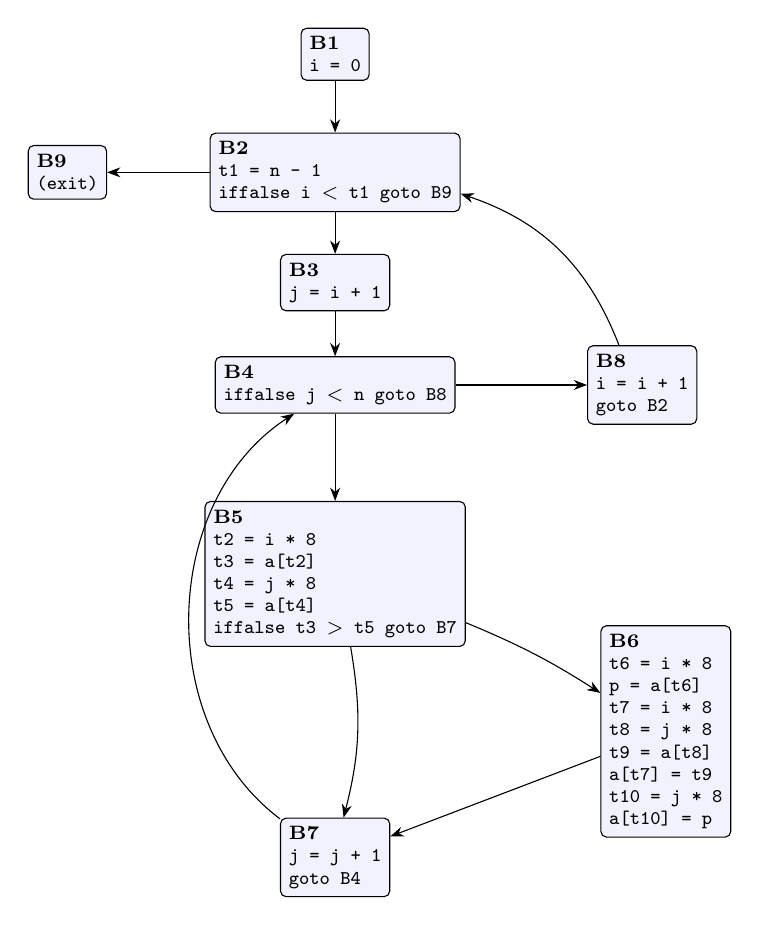
\begin{tikzpicture}[>=Stealth,font=\scriptsize,x=1.000cm,y=1.000cm,
 box/.style={draw,rounded corners=2pt,align=left,inner sep=3pt,fill=blue!5},
 circ/.style={draw,circle,align=center,inner sep=1pt,minimum size=0.75cm,fill=blue!5},
 lab/.style={font=\scriptsize,inner sep=1pt,fill=white,fill opacity=0.85,text opacity=1}]
\node[box] (b1) at (0.000,0.000) {\textbf{B1}\\\texttt{i = 0}};
\node[box] (b2) at (0.000,-1.500) {\textbf{B2}\\\texttt{t1 = n - 1}\\\texttt{iffalse i \textless{} t1 goto B9}};
\node[box] (b3) at (0.000,-2.900) {\textbf{B3}\\\texttt{j = i + 1}};
\node[box] (b4) at (0.000,-4.200) {\textbf{B4}\\\texttt{iffalse j \textless{} n goto B8}};
\node[box] (b5) at (0.000,-6.600) {\textbf{B5}\\\texttt{t2 = i * 8}\\\texttt{t3 = a[t2]}\\\texttt{t4 = j * 8}\\\texttt{t5 = a[t4]}\\\texttt{iffalse t3 \textgreater{} t5 goto B7}};
\node[box] (b6) at (4.200,-8.600) {\textbf{B6}\\\texttt{t6 = i * 8}\\\texttt{p = a[t6]}\\\texttt{t7 = i * 8}\\\texttt{t8 = j * 8}\\\texttt{t9 = a[t8]}\\\texttt{a[t7] = t9}\\\texttt{t10 = j * 8}\\\texttt{a[t10] = p}};
\node[box] (b7) at (0.000,-10.200) {\textbf{B7}\\\texttt{j = j + 1}\\\texttt{goto B4}};
\node[box] (b8) at (3.900,-4.200) {\textbf{B8}\\\texttt{i = i + 1}\\\texttt{goto B2}};
\node[box] (b9) at (-3.400,-1.500) {\textbf{B9}\\\texttt{(exit)}};
\draw[->] (b1) --  (b2);
\draw[->] (b2) --  (b3);
\draw[->] (b2) --  (b9);
\draw[->] (b3) --  (b4);
\draw[->] (b4) --  (b5);
\draw[->] (b4) --  (b8);
\draw[->] (b5) to[bend left=5]  (b6);
\draw[->] (b5) to[bend left=12]  (b7);
\draw[->] (b6) --  (b7);
\draw[->] (b7) to[bend left=55]  (b4);
\draw[->] (b8) to[bend right=25]  (b2);
\end{tikzpicture}
\end{document}
